

\chapter{ROS Graphs}
\label{app:ros2graphs}
In ROS, the communication between nodes is facilitated through a system of topics, services, and actions. The ROS 2 graph is a representation of this communication network, showing how nodes are connected and how they exchange messages.
Here are some ROS graphs from different stages of the engineering.

\section{ROS Graph of the Mapping Stage}
\label{subsec:rosgraph_mapping}
\newgeometry{left=2cm,right=1cm,top=1cm,bottom=0.05cm}
\begin{landscape}
    \thispagestyle{empty}
    \begin{figure}[p]
        \centering
        
\includegraphics[height=0.69\textwidth]{figs/ros_graphs/mapping_stage_rosgraph.png}
        \caption{ROS Graph of the Mapping Stage}
        \label{fig:rosgraph_mapping}
    \end{figure}
\end{landscape}
\restoregeometry

\section{ROS Graph of the Localization Stage}
\label{subsec:rosgraph_localization}
\newgeometry{left=1cm,right=2.9cm,top=1cm,bottom=1cm}
\begin{landscape}
    \thispagestyle{empty}
    \begin{figure}[p]
        \centering
        
\includegraphics[height=0.75\textwidth]{figs/ros_graphs/localization_stage_rosgraph.png}
        \caption{ROS Graph of the Localization Stage}
        \label{fig:rosgraph_localization}
    \end{figure}
\end{landscape}
\restoregeometry

\section{ROS Graph of the Navigation Stage}
\label{subsec:rosgraph_navigation}
\newgeometry{left=0.5cm,right=3.6cm,top=1cm,bottom=0.05cm}
\begin{landscape}
    \thispagestyle{empty}
    \begin{figure}[p]
        \centering
        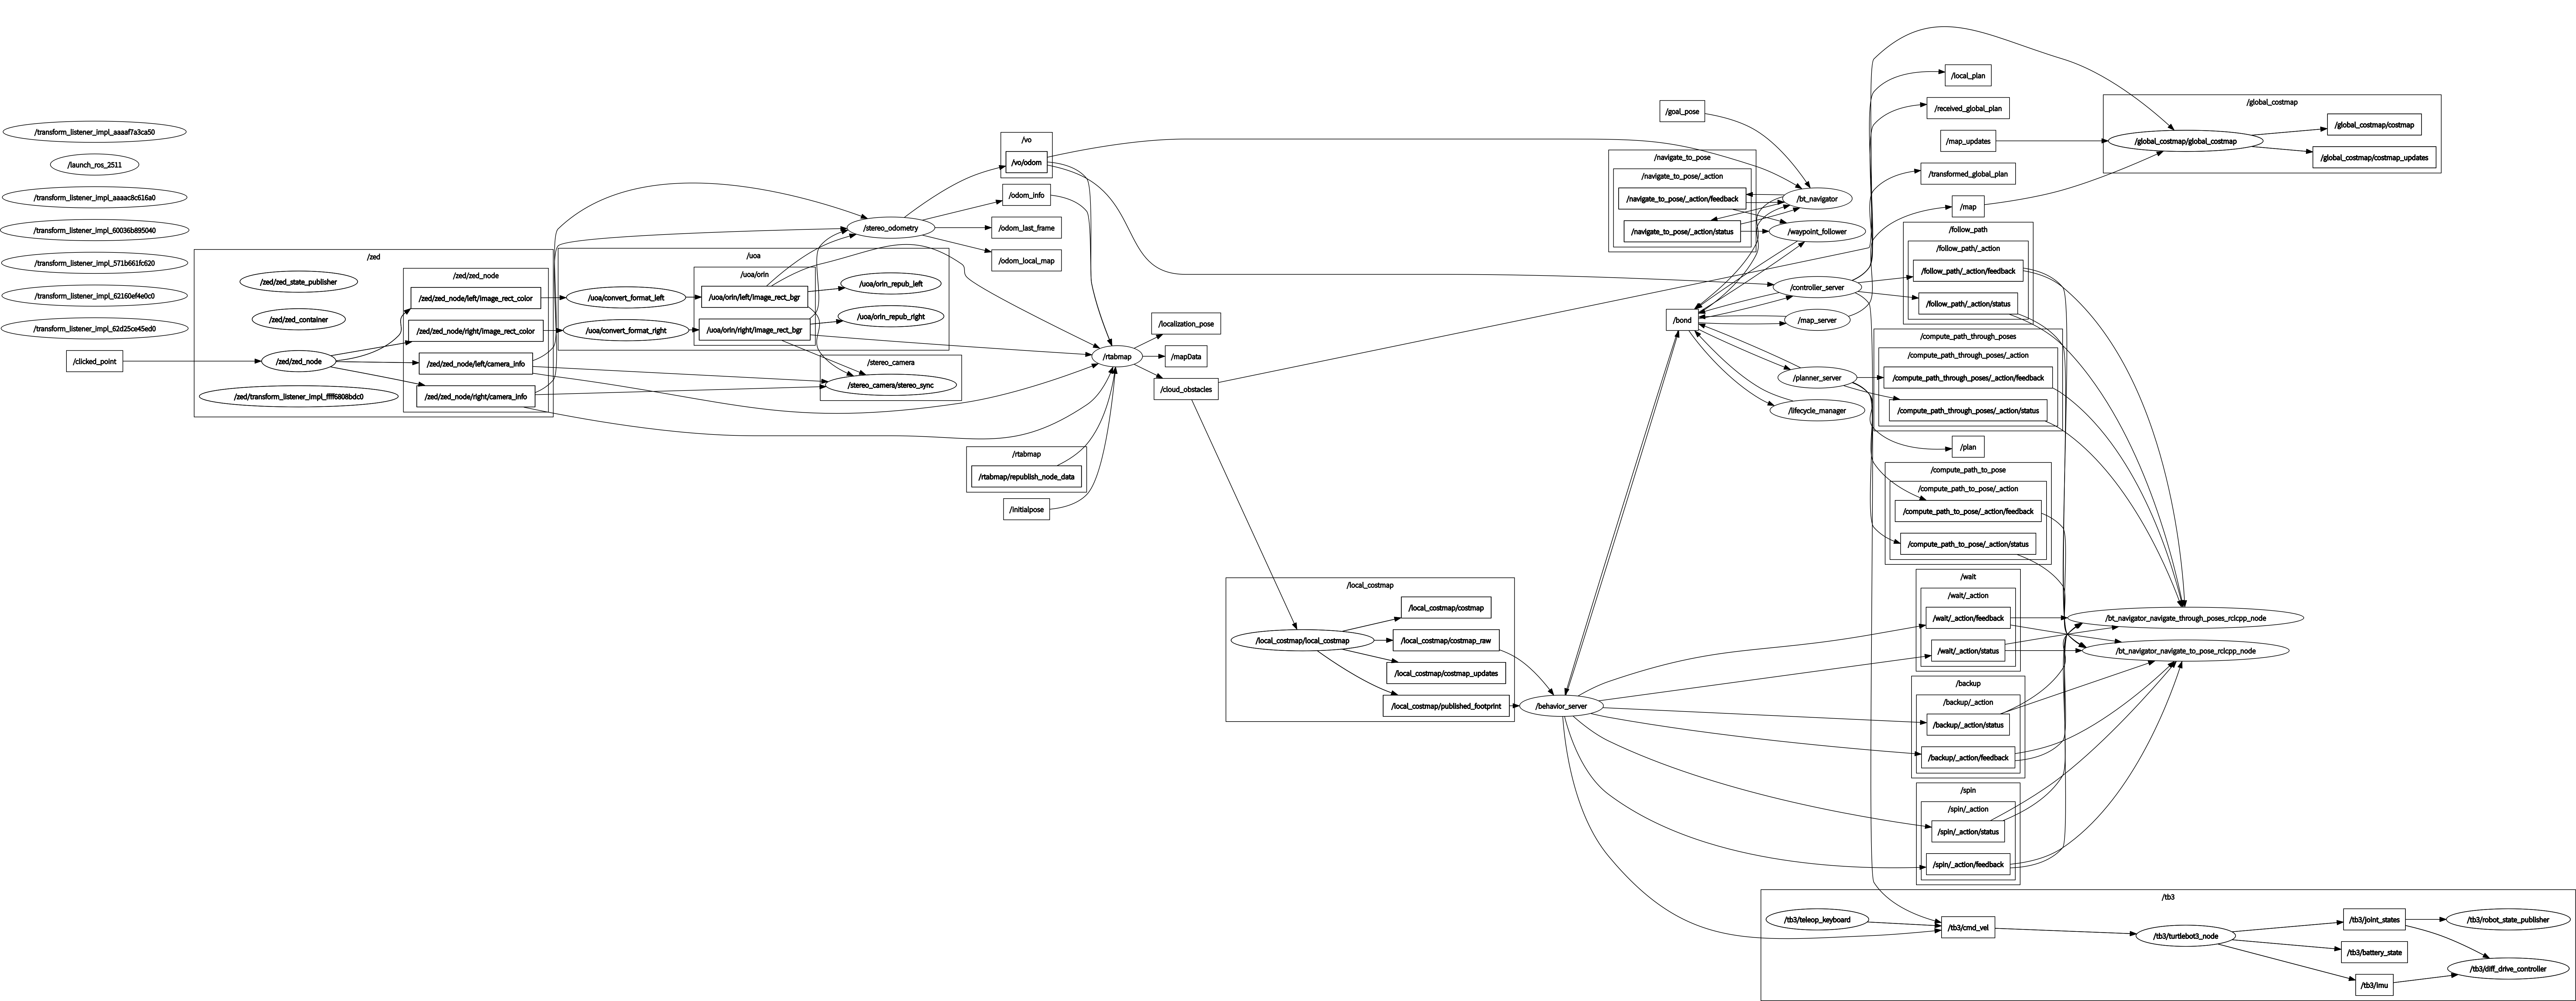
\includegraphics[height=0.68\textwidth]{figs/ros_graphs/navigation_stage_rosgraph.png}
        \caption{ROS Graph of the Navigation Stage}
        \label{fig:rosgraph_navigation}
    \end{figure}
\end{landscape}
\restoregeometry
